\documentclass[12pt]{article}
\usepackage[utf8]{inputenc}
\usepackage[russian]{babel}
\usepackage{hyperref}
\usepackage{color}
\usepackage{amssymb}
\usepackage{amsmath}
\usepackage{graphicx}
\usepackage{tikz}
\usepackage{titling}
\usepackage{lipsum}
\usepackage{titlesec}

\titlespacing\section{0pt}{10pt plus 2pt minus 2pt}{0pt plus 2pt minus 2pt}

\setlength{\droptitle}{-10em}   % This is your set screw

\author{Михаил Лепехин и Роман Логинов, группа 694}
\title{Online Convex Optimization (OCO)}

\begin{document}
  \maketitle

\section*{Применение Online Convex Optimisation к задаче фильтрации спама}
$ $

Предположим, что признаки email-сообщений принадлежат множеству $\mathcal{X}$. В качестве признаков будем рассматривать частоты вхождений слов (или групп слов, чтобы размерность мн-ва признаков не получилась слишком большой) в сообщение.

На каждом шаге $t$ функция $a_t : \mathcal{X} \rightarrow [0, 1]$, сопоставляет вектору $x \in \mathcal{X}$ значений признаков некоторое число из отрезка $[0, 1]$. По смыслу это значение является оценкой вероятности (уверенности) того, что сообщение с данными значениями признаков является спамом.

На каждом шаге $t$ соперник выбирает вектор значений признаков $x_t$ и индикатор $y_t$ того, что данное сообщение является спамом.

Для оценки точности метода принятия решений $a_t$ нужно взять некоторую функцию потерь $f_t$. Например, квадратичную функцию потерь:

$$f_t(a_t) := (y_t-a_t(x_t))^2.$$

На каждом шаге функция $a_t(x)$ выбирается из некоторого множества так, чтобы минимизировать $regret$:

$$\sum\limits_{t=1}^T f_t(a_t) - \min\limits_{a \in \mathcal{A}} \sum\limits_{t=1}^T f_t(a) = \sum\limits_{t=1}^T (y_t-a_t(x_t))^2 - \min\limits_{a \in \mathcal{A}} \sum\limits_{t=1}^T (y_t-a(x_t))^2$$

\section*{Выбор функции $a_t(x)$}
$ $


В машинном обучении для решения задачи классификации спама часто делают следующее. При помощи некоторого алгоритма находят вектор фильтра $a$ из шара $B_R(0)$ относительно некоторой нормы. А после - для определения, является ли сообщение с вектором значений признаков $x$ спамом, рассматривают скалярное произведение $<a, x>$.

Если $<a, x>$ > 0, то сообщение является спамом. Если же знак скалярного произведения отрицательный, то сообщение не является спамом. А если получилось так, что скалярное произведение равно 0, то считается, что тип сообщения не определён.

Будем строить функцию $a_t$ из похожих соображений. Будем также подбирать вектор фильтра $w_t$ из $W := B_R(0)$ и большим значениям скалярного произведения $<w_t, x>$ будет сопоставлять большую вероятность.

В качестве $\mathcal{X}$ возьмём множество векторов $x$ из $\mathbb{R_{+}}^d$, что $\sum\limits_{i=1}^n x_i = 100$ (здесь каждой группе слов сопоставляется процент количества слов из этой группы по отношению ко всем словам в сообщении).

Покажем, что скалярного произведение $<w_t, x>$ ограничено. По неравенству Коши-Буняковского:

$$<w_t, x>^2 \leq ||w_t||_2^2*||x||_2^2 \leq R^2*||x||_2^2 \leq R^2*100^2.$$

Причём, равенство здесь достигается, если сразу выполняются 3 ограничения:

1) $x$ коллинеарен $w_t$ - получим равенство в нер-ве К-Б,

2) $w_t=R$ - получим 2 равенство,

3) $\exists i \in \{1, \dots, d\}: x_i = 100$.

Тогда определим $M := 100R$.

В качестве функции $a_t(x)$ возьмём

 $$a_t(x) = \frac{<x, w_t>+M}{2M}.$$
 
 Тогда функция $f_t$ запишется следующим образом:
 
 $$f_t(x) = \bigg(y_t - \frac{<x, w_t>+M}{2M}\bigg)^2$$
 
\section*{Свойства выбранной функции $a_t(x)$}
$ $

Для нас очень важным свойством будет являться то, что выбранная функция $a_t(x)$ выпукла. Покажем это.

Вычислим её градиент.

$$\frac{\partial f_t}{\partial x}(x) = \frac{2}{2M}(<x, w_t>+M)\frac{w_t}{2M} = \frac{<x, w_t>+M}{2M^2}w_t$$

Продифференцируем градиент по $x$ и получим гессиан.

$$\frac{\partial^2 f_t}{\partial x^2}(x) = \frac{1}{2M^2}w_tw_t^T \succeq 0$$

Положительная полуопределённость следует из того, что $\forall x \in \mathcal{X}: x^Tw_tw_t^Tx_t = (w_t^Tx_t)^Tw_t^Tx_t = <w_t^Tx_t, w_t^Tx_t> \geq 0$ - по свойствам скалярного произведения.

По дифференциальному критерию выпуклости 2 порядка функция $f_t(x)$ выпукла. 

\section*{Вычисление regret}
$ $

Для того, чтобы проверять качество работы методов, очень полезно уметь получать значение $regret$.

С учётом выбора функции $a_t(x)$ $regret$ можно записать следующим образом:

$$\sum\limits_{t=1}^T (y_t-a_t(x_t))^2 - \min\limits_{a \in \mathcal{A}} \sum\limits_{t=1}^T (y_t-a(x_t))^2 =$$
$$= \sum\limits_{t=1}^T\bigg(y_t - \frac{<x_t, w_t>+M}{2M}\bigg)^2 - \min\limits_{w \in W}\sum\limits_{t=1}^T\bigg(y_t - \frac{<x_t, w>+M}{2M}\bigg)^2$$

При этом заметим, что $\forall t=1, \dots, T: g_t(w) = \bigg(y_t - \frac{<x_t, w>+M}{2M}\bigg)^2$ является выпуклой по $w$ (доказательство аналогично выпуклости $f_t$ по $x$).
Значит, функция $g(w) = \sum\limits_{t=1}^T\bigg(y_t - \frac{<x_t, w>+M}{2M}\bigg)^2$ является выпуклой как сумма выпуклых функций.

Чтобы получить точное или приближённое значение $regret$ нужно точно или приближённо решить следующую задачу оптимизации:

$$\min g(w)$$
$$s.t. w \in W$$

Эта задача является выпуклой, поскольку:

1) $g(w)$ выпукла в $\mathbb{R}^d$, как было показано выше;

2) множество $W = B_0(R)$ выпукло, поскольку любые 2 точки, лежащие в шаре можно соединить отрезком, каждая точка которого будет также принадлежать этому шару.


Поэтому для получения точного значения $regret$ можно применить теорему Каруша-Куна-Таккера. В силу выпуклости задачи  оптимизации стационарные точки лагранжиана будут точками минимума функции. 

Но нам вполне хватит и приближённого означения $regret$, поэтому для решения вспомогательной задачи оптимизации воспользуемся пакетом $cvxpy$.

\section*{Методы первого порядка}
$ $

В данном разделе мы рассмотрим базовые алгоритмы для Online Convex Optimization, которые достаточно неплохо применимы на практике.

В целом данные методы похожи на соответствующие методы первого порядка для задач обычной выпуклой оптимизации. Но они принципиально отличаются целью применения. Ведь при помощи методов OCO мы стремимся минимизировать не ошибку оптимизации, а \textit{regret}:

$$regret = \sum\limits_{t=1}^T f_t(x_t) - \min\limits_{x \in \mathcal{K}} \sum\limits_{t=1}^T f_t(x)$$

Для сравнения $regret$ с ошибкой оптимизации полезно рассмотреть среднее значение $regret$, т.е. $\frac{regret}{T}$.

Введём обозначение:

$$\overline{x}_T := \frac{1}{T}\sum\limits_{t=1}^T x_t$$

Пусть все функции $f_t$ равны некоторой функции $f : \mathcal{K} \rightarrow \mathbb{R}$, то из неравенства Йенсена получим:

$$f(\overline{x}_T)-f(x^*) = f(\overline{x}_T)- \frac{1}{T} \sum\limits_{t=1}^T f(x^*) \leq \frac{1}{T}\sum\limits_{t=1}^T \big(f(x_t)-   f(x^*)\big	)$$

Таким образом мы показали следующий факт: 

функция $f(x_T)$ сходится к $f(x*)$ не менее быстро, чем среднее значение $regret$.

\section*{Online gradient descent}
$ $

Этот алгоритм, пожалуй, является одним из наиболее интуитивных и простых в Online Convex Optimization. Он базируется на известном нам методе градиентного спуска для offline выпуклой оптимизации.

На каждой итерации этот алгоритм делает шаг от предыдущей точки $x_k$ в направлении градиента предыдущего веса. Но такой шаг может привести к выходу за границу допустимого выпуклого множества $D$. Для того, чтобы этого не произошло, алгоритм проецирует полученную точку обратно на множество $D$, находя ближайшую к ней в $D$.

Псевдокод алгоритма.

Вход: выпуклое множество $\mathcal{K}$, $T$ - размер выборки, $x_1 \in \mathcal{K}$ - начальное приближение, массив со значениями размеров шагов $\alpha_t$.

$\textbf{for}$ $t = 1 \dots T$ $\textbf{do}$

$\textbf{begin}$

$\quad$ Получить $x_t$ и найти значение $f_t(x_t)$

$\quad$ Сделать шаг градиентного спуска.

$\quad y_{t+1} = x_t - \alpha_t \nabla f_t(x_t)$

$\quad$ Спроецировать полученную точку на допустимое выпуклое множество $\mathcal{K}$.

$\quad x_{t+1} = Pr_{\mathcal{K}}(y_{t+1})$

$\textbf{end}$

Выход: значение $x_{T+1}$.

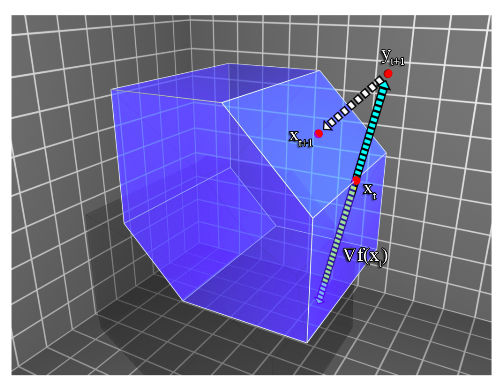
\includegraphics[width=\linewidth]{gradient_descent.png}

\subsubsection*{Нахождение проекции на допустимое множество}

При решении нашей задачи нам нужно будет искать проекцию точки $y_{t+1}$ на $\mathcal{K}$, являющееся шаром радиуса $R$ по евклидовой норме.

Покажем, как это делается.

Нужно решить следующую задачу оптимизации:

$$min ||y-x||_2^2$$
$$s.t.\ x^Tx = R^2$$

Перезапишем квадрат евкидовой нормы в удобном нам виде.

$$min (y-x)^T(y-x)$$
$$s.t.\ x^Tx = R^2$$

1) Если $y_{t+1} \in \mathcal{K}$, то $Pr_{\mathcal{K}}(y) = y$.

2) Решим задачу оптимизации при помощи теоремы ККТ.

	Эта задача выпукла, так как допустимое множество выпукло и оптимизируемая функция является выпуклой как композиция выпуклой и неотрицательной (евклидова норма) и строго возрастающей на неотрицательных значениях ($h(t) = t^2$).
	Значит, найденная стационарная точка лагранжиана даст глобальный условный минимум функции $||y-x||_2^2$.
	
	Итак, запишем лагранжиан.
	
	$$L(x, \mu) = (y-x)^T(y-x) + \mu(x^Tx - R^2)$$	
	
	Для нахождения его стационарных точек, посчитаем градиент.
	
	$$\frac{\partial L}{\partial x}(x, \mu) = 2(1+\mu)x - 2y$$
	
Запишем условие	стационарности.
	
	$$2(1+\mu)x - 2y = 0\ (*)$$ 
	
	Вспомним следующее условие ККТ:
	
	$$\mu(x^Tx-R^2) = 0$$
	
	Это возможно в 2 случаях:
	
	1) $\mu = 0$, откуда из $(*)$ следует $x=y$, что невозможно, так как $y$ не принадлежит допустимому множеству.
	
	2) $x^Tx = R^2$
	
	Значит, $x$ лежит на границе шара $\mathcal{K}$.
	
	Заметим, что все условия ККТ, в том числе, и равенство 0 градиента лагранжиана, выполняются при выборе $x = \frac{y}{||y||_2}$.
	
	Значит, в качестве проекции будем брать именно эту точку.

\subsection{Оценки для online градиентного спуска}
$ $

Будем предполагать градиент каждой из функций $f_t$ ограниченным с константой $G$ (для всего семейства функций).

А также будем рассматривать поведение online градиентого спуска на ограниченных множествах с диаметром $D$ (в нашей задаче используется шар радиуса $R$. Его диаметр равен $2D$).

Несмотря на то, что функция весов на каждом следующем шаге может существенно отличаться от веса на предыдущем шаге, $regret$, получаемый алгоритмом все равно будет сублинейным.

$ $

Это следует из следующей теоремы.

\textbf{Теорема.} Online градиентный спуск с шагом, заданным по правилу $\alpha_t = \frac{D}{G\sqrt{t}}$, для любого $T \geq 1$ гарантирует:

$$regret = \sum\limits_{t=1}^T f_t(x_t) - \min\limits_{x\in \mathcal{K}} \sum\limits_{t=1}^T f_t(x) \leq \frac{3}{2}GD\sqrt{T}$$

$ $

Эта теорема очень важна, поскольку обосновывает применимость метода online градиентного спуска в данной задаче.

Поэтому докажем её.

\textbf{Доказательство.}

Здесь в качестве нормы $||.||$ будем использовать стандартную евклидову норму $||.||_2$.

При доказательстве будем пользоваться следующим вспомогательным утверждением.

\textbf{Утверждение. (Теорема Пифагора)} Пусть $\mathcal{K} \subset \mathbb{R}^d$ - выпуклое множество, $y \in \mathbb{R}^d$ и $x=Pr_{\mathcal{K}}(y)$. Тогда $\forall z \in \mathcal{K}: ||y-z|| \geq ||x-z||$.

Пусть $x^* \in arg \min\limits_{x \in \mathcal{K}} \sum\limits_{t=1}^T f_t(x)$.

Определим $d_t := \nabla f_t(x_t)$.

Из выпуклости функции $f_t(x)$ и дифференциального критерия выпуклости 1 порядка получим:

$$f_t(x_t) - f_t(x^*) \leq d_t^T (x_t-x^*).\ (1)$$

По теореме Пифагора получим:

$$||x_{t+1}-x^*||^2 = ||\Pr_{\mathcal{K}}(x_t - \alpha_td_t) -x^*||^2 \leq ||x_t-\alpha_t d_t-x^*||^2\ (2)$$

Отсюда по неравенству треугольника:

$$||x_{t+1}-x^*||^2 \leq ||x_t-x^*||^2 + \alpha_t^2||d_t||^2 - 2\alpha_td_t^T(x_t-x^*)$$

Учитывая, что $||d_t|| \leq G$ (такое предположение мы делали в самом начале пункта), получим следующую верхнюю оценку.

$$2d_t^T(x_t-x^*) \leq \frac{||x_t-x^*||^2 - ||x_{t+1}-x^*||^2}{\alpha_t} + \alpha_t G^2\ (3)$$ 

Просуммируем неравенства (1) и (3) по $t=1, \dots, T$ и с учётом выбора шага $\alpha_t = \frac{D}{G\sqrt{T}}$, получим:

$$2\bigg(\sum\limits_{t=1}^T f_t(x_t) - f_t(x^*) \bigg) \leq 2\sum\limits_{t=1}^T d_t^T(x_t-x^*) \leq \sum\limits_{t=1}^T 
\bigg(\frac{||x_t-x^*||^2 - ||x_{t+1}-x^*||^2}{\alpha_t} + \alpha_t G^2\bigg)$$
$$= \sum\limits_{t=1}^T 
\frac{||x_t-x^*||^2 - ||x_{t+1}-x^*||^2}{\alpha_t} + G^2 \sum\limits_{t=1}^T \alpha_t \leq $$
$$\leq \sum\limits_{t=1}^T 
||x_t-x^*||^2*\bigg(\frac{1}{\alpha_t}-\frac{1}{\alpha_{t-1}}\bigg) + G^2 \sum\limits_{t=1}^T \alpha_t $$

При последнем неравенстве для удобства положим $\frac{1}{\alpha_0} = 0$

$$\sum\limits_{t=1}^T 
||x_t-x^*||^2*\bigg(\frac{1}{\alpha_t}-\frac{1}{\alpha_{t-1}}\bigg) + G^2 \sum\limits_{t=1}^T \alpha_t \leq $$
$$\leq D^2\sum\limits_{t=1}^T \bigg(\frac{1}{\alpha_t}-\frac{1}{\alpha_{t-1}}\bigg) + G^2 \sum\limits_{t=1}^T \alpha_t = D^2 \frac{1}{\alpha_T} + G^2 \sum\limits_{t=1}^T \alpha_t$$

И, наконец, из выбора шага и того факта, что $\sum\limits_{t=1}^T \frac{1}{\sqrt{t}} \leq 2\sqrt{T}$:

$$D^2 \frac{1}{\alpha_T} + G^2 \sum\limits_{t=1}^T \alpha_t \leq 3DG\sqrt{T}$$
\textbf{Теорема доказана.}

$ $

Кроме того, при выборе шага по данному правилу метод online градиентного спуска является асимптотически оптимальным по значению $regret$.

\textbf{Теорема.} Любой алгоритм для OCO в худшем случае выдаёт $regret = \Omega(DG\sqrt{T})$. Это утверждение верно даже при выборе функции веса из некоторого фиксированного распределения.

$ $

Также стоит отметить, что online gradient descent даёт гораздо более точный результат на сильно выпуклых функциях. Об этом можно судить по следующей теореме.
$ $

\textbf{Теорема.} Для сильно выпуклых функций потерь с константой $\mu$ $online$ градиентный спуск с шагом, выбранным по правилу $\alpha_t = \frac{1}{\mu t}$, гарантирует следующую верхнюю оценку для $regret_T$:

$$regret_{T} \leq \frac{G^2}{2\mu}(1 + log\ T).$$

\section*{Stochastic online gradient descent}
$ $

Одним из случаев online выпуклой оптимизации является стохастическая оптимизация. Как и в стандартной оптимизации, при стохастической оптимизации оптимизатор стремится минимизировать выпуклую функцию $f$, заданную на выпуклом множестве $\mathcal{K}$.

$$\min f(x)$$
$$s.t.\ x \in \mathcal{K}$$

Но в отличие от стандартной оптимизации, алгоритм работает не с градиентом $\nabla_x$ оптимизируемой функции напрямую, а с стохастическим (или зашумлённым) градиентом $\widehat{\nabla}_x$, который является случайной величиной.

При этом, на стохастический градиент накладываются следующие ограничения:
   
1) Несмещённость

   $$\textbf{E}\widehat{\nabla}_x = \nabla f(x)$$
   
2) Ограниченность в среднем

   $$\textbf{E}[\widehat{\nabla}_x^2] \leq G^2$$

*) Для хороших оценок сходимости часто требуют липшициевость стохастического градиента

   $$\widehat{\nabla}_x = O(x)$$

Псевдокод метода online стохастического градиентного спуска.

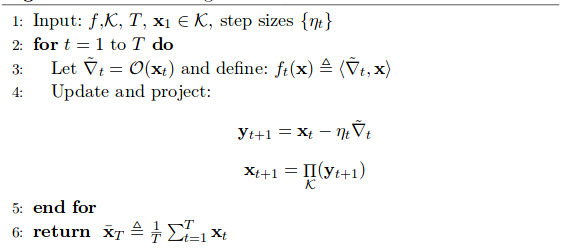
\includegraphics[width=\linewidth]{SGD_algo.png}

Применимость стохастического градиентного спуска в нашей задаче показывает следующая теорема.

\textbf{Теорема.} Стохастический градиентный спуск с размером шага $\alpha_t = \frac{D}{G\sqrt{T}}$ гарантирует:

$$\textbf{E}[f(\overline{x}_T)] \leq \min\limits_{x^* \in \mathcal{K}} f(x^*) + \frac{3GD}{2\sqrt{T}}$$


\end{document}